\section*{Exercice 8~: L'utilisation des réseaux de Pétri pour le
  contrôle des trains}
  
\emph{Nous suiverons ici le schema, qui représente 6 secteurs allant
  de 1 à 6, et non l'énoncé, qui évoque 7 secteurs de 1 à 7. Pour la
  question 3 les secteurs seront, par simplicité de notation, supposés
  numérotés de 0 à n et non de 1 à n+1.}

\subsection*{Question 1}

Chaque place pourra correspondre à un secteur, chaque jeton à un train
et chaque transition est un mouvement de train d'un secteur au
prochain secteur~:

\begin{center}
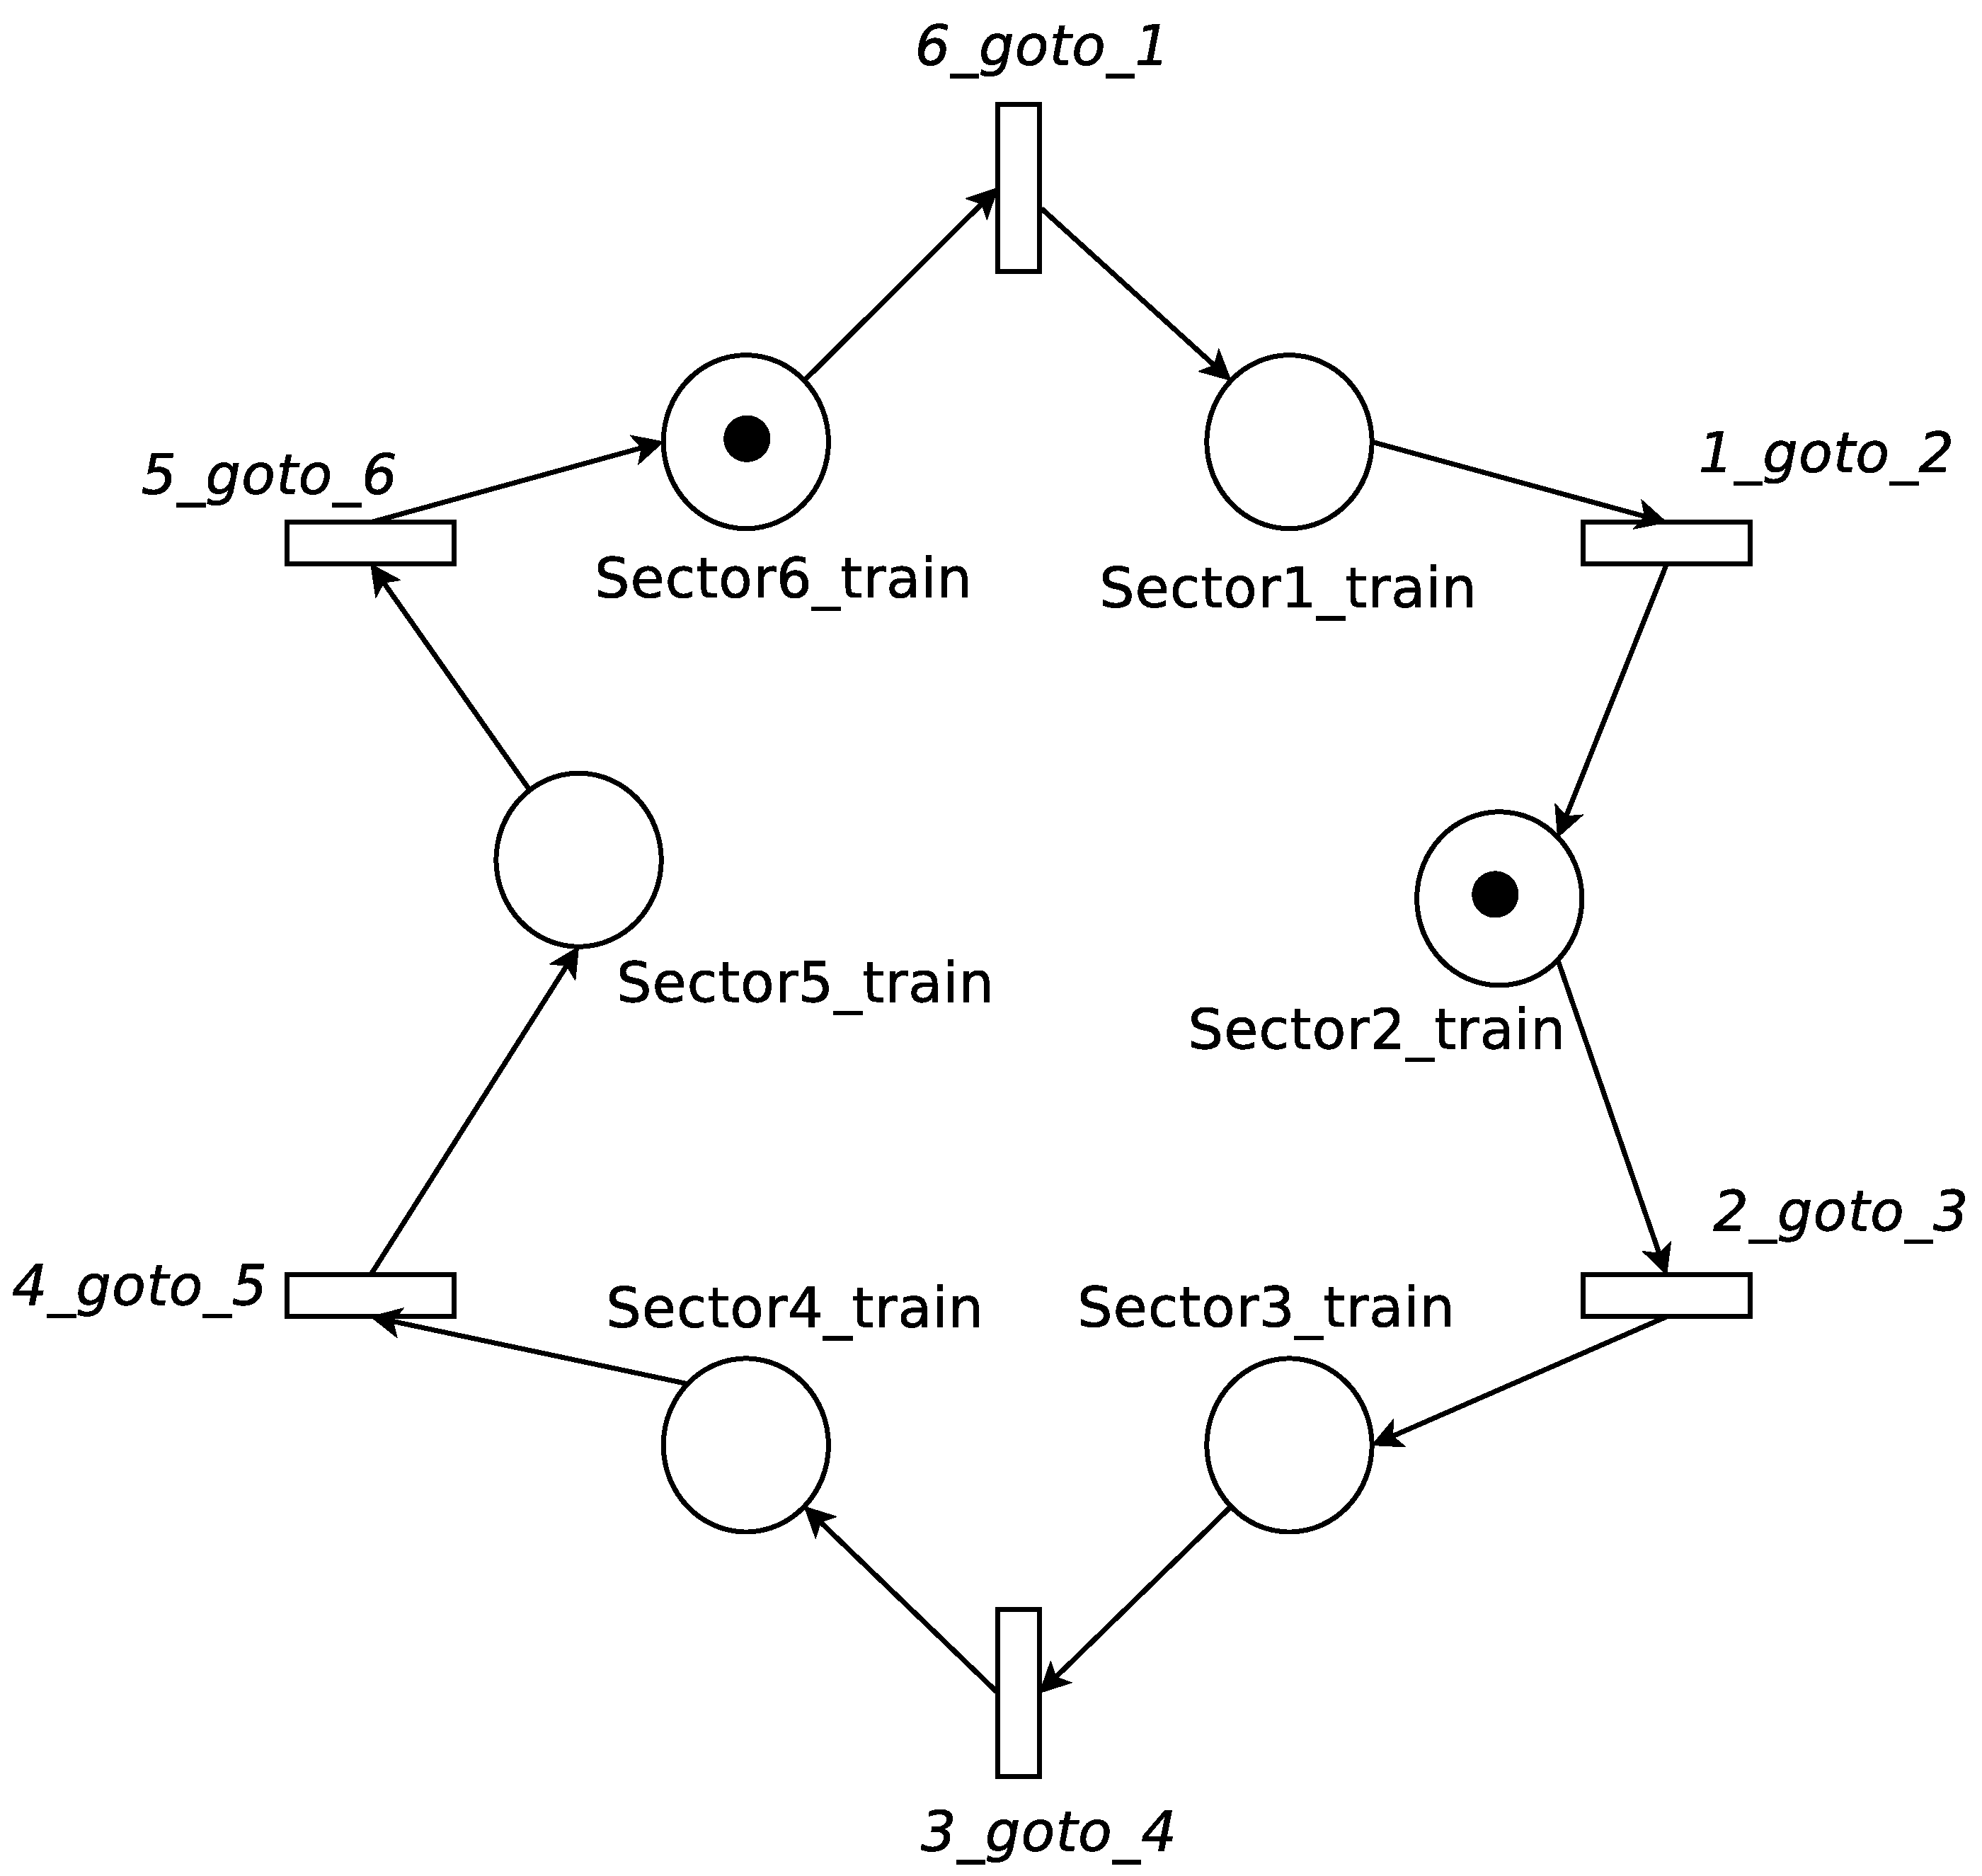
\includegraphics[height = 0.3\paperwidth]{exo8_1.eps}
\end{center}

Le réseau ci-dessus n'empêche cependant pas la collision de trains,
chose qu'il serait préférable d'éviter. Démunis d'arcs inhibiteurs,
nous nous devions de créer pour chaque secteur une place binaire dont
la présence d'un jeton correspond à la non présence de train dans ce
secteur.

\emph{Les parties ajoutées sont en vert~:}

\begin{center}
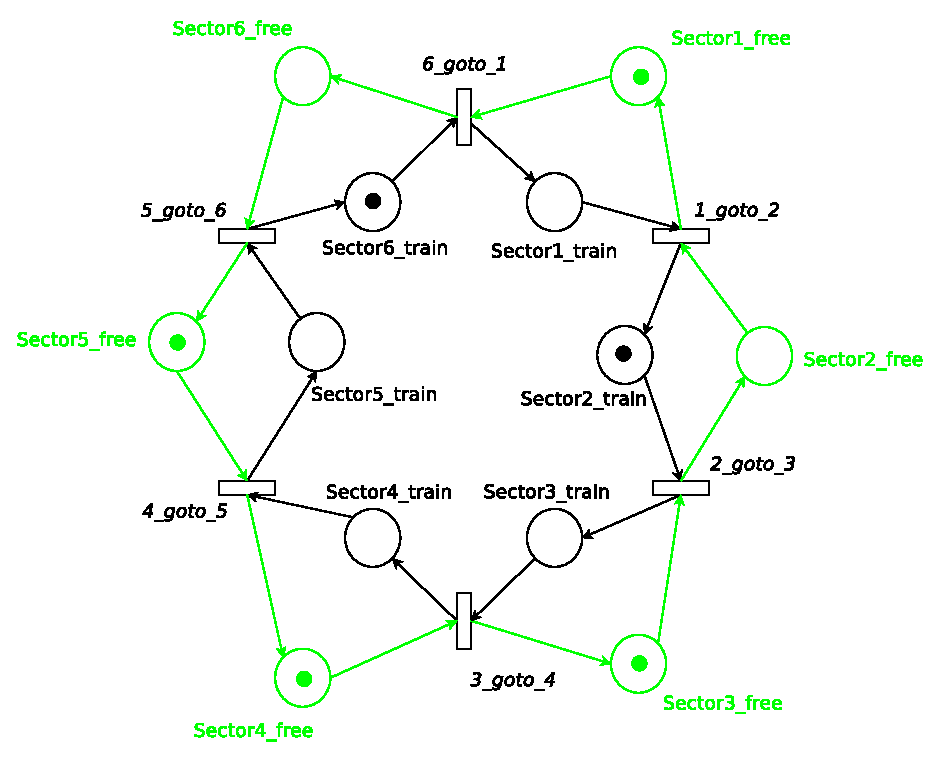
\includegraphics[height = 0.4\paperwidth]{exo8_2.eps}
\end{center}

Nous avons ainsi comme invariant qu'un secteur est toujours soit
libre, soit occupé par un seul et unique train. Il nous reste comme
condition à remplir que les secteurs adjacents à un secteur occupé
soient libres~:

\begin{center}
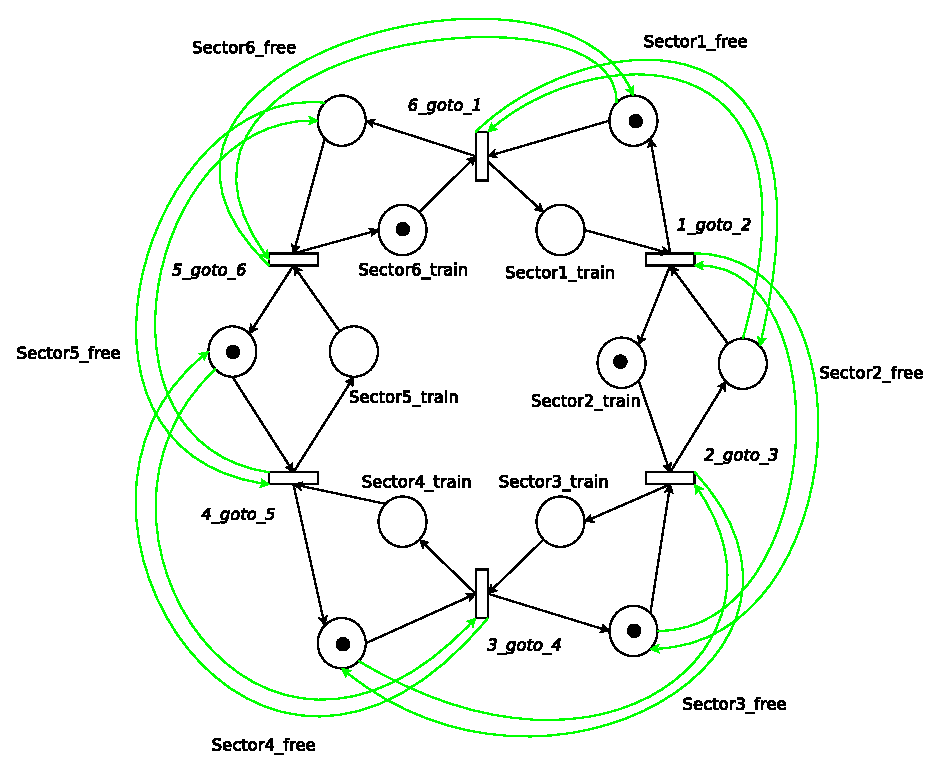
\includegraphics[height = 0.5\paperwidth]{exo8_3.eps}
\end{center}

Maintenant il faut différencier les deux trains, chose que nous
pouvons faire en recopiant le cycle interne de places.

\emph{Pour faciliter la lecture, les deux circuits analogiques pour
  les deux trains ont étés coloriés en rouge et en bleu
  respectivement~:}

\begin{center}
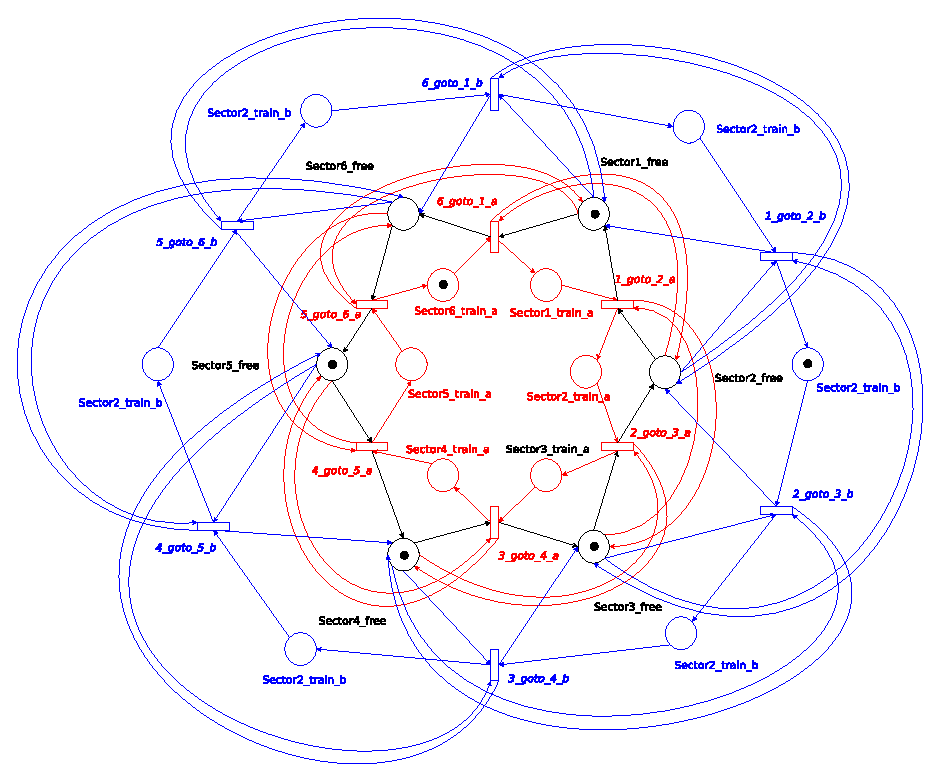
\includegraphics[height = 0.6\paperwidth]{exo8_uncoloured.eps}
\end{center}


\subsection*{Question 2}

En partant du réseau précédent et en écrasant les deux circuits
\og{}train\fg{} en un seul, nous nous retrouvons avec le réseau
colorié suivant.

\emph{Le jeton rouge représente le premier train, le bleu la deuxième, et ceux
noirs l'absence de train pour un secteur donné~:}

\begin{center}
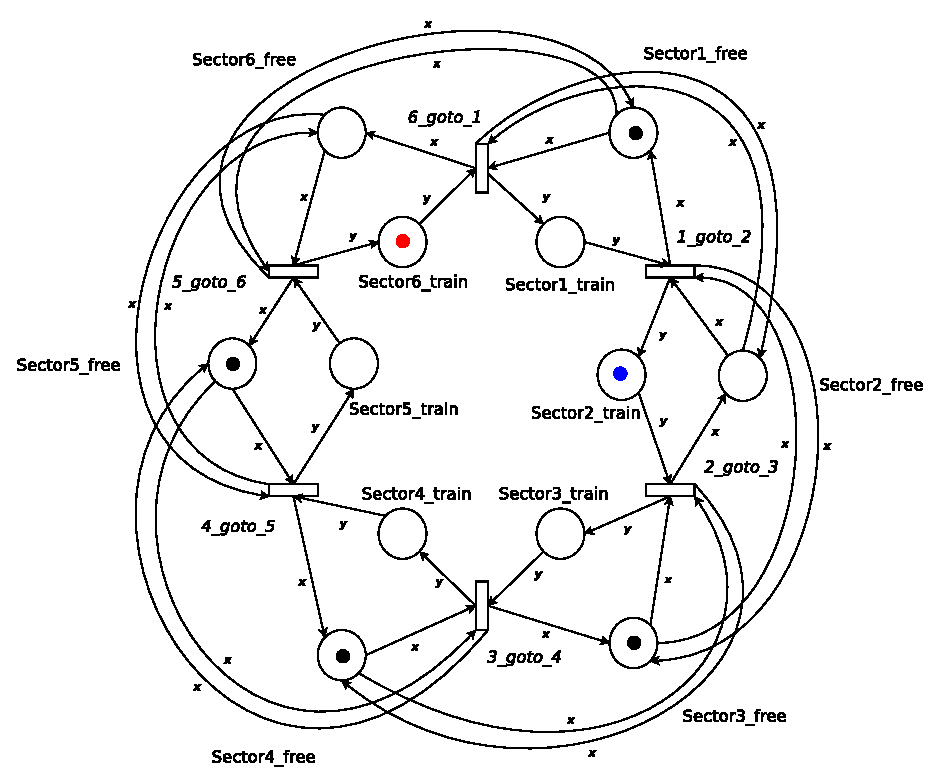
\includegraphics[height = 0.5\paperwidth]{exo8_coloured.eps}
\end{center}

Il est possible de simplifier ce réseau en écrasant les deux cycles ensemble. 
Ci-dessous un jeton noir correspond à la non-présence d'un train dans le secteur 
correspondant, un jeton d'une autre couleur à un train présent~:

\begin{center}
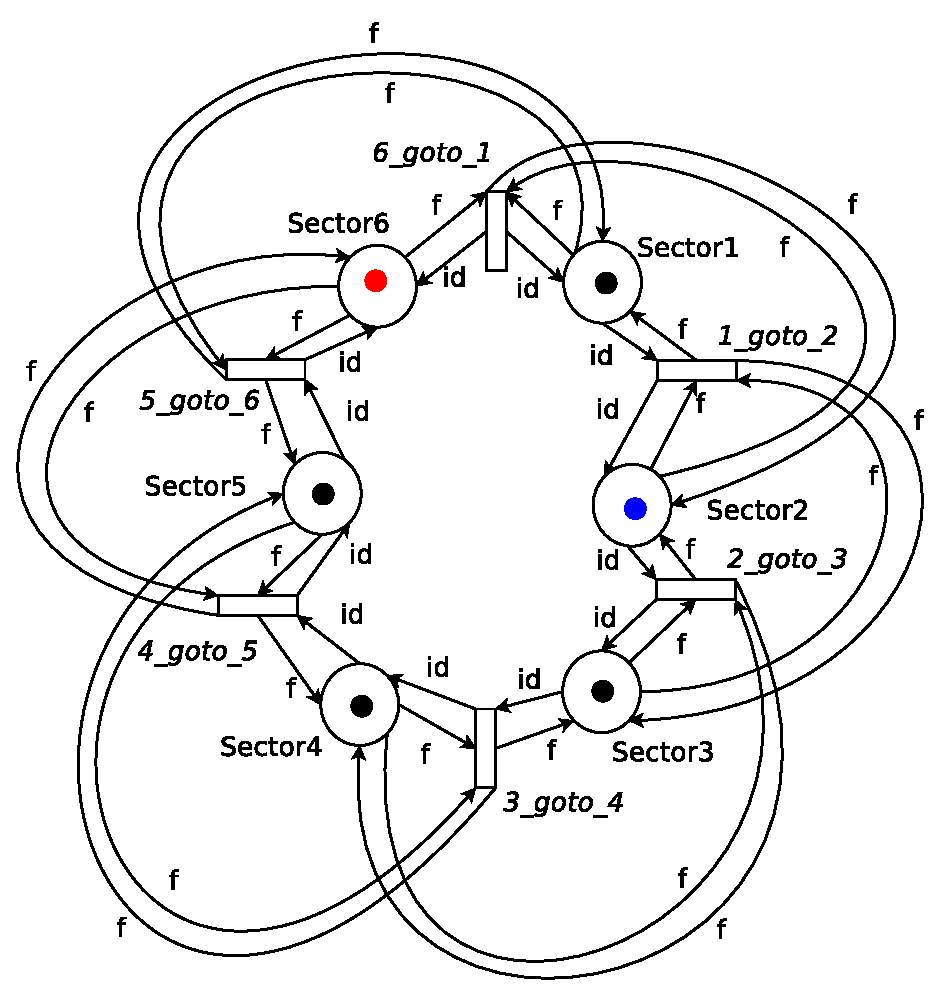
\includegraphics[height = 0.5\paperwidth]{exo8_coloured_2_v2.eps}
\end{center}

Où~:

$\forall c \in \{RED, BLUE\}$ $id(c) = c$

$\forall c \in \{RED, BLUE\}$ $f(c) = BLACK$

Ce réseau est beaucoup plus simple à aborder que la version
non-colorée, qui pour $n$ trains aura $n+1$ fois plus de places. Cela
étant sans la définition de la fonction $f$ (projection sur la couleur
noir) il n'est pas possible de comprendre le fonctionnement du
réseau~: le prix de la simplification du graphe est une augmentation
de la complexité des fonctions de transition.

Le premier réseau coloré semble un bon compromis entre les deux~: le
graphe a du sens sans information supplémentaire, mais reste un
facteur linéaire (en le nombre de trains) plus \og{}compact\fg{} que le réseau
non-coloré.


\subsection*{Question 3}

Soit le réseau suivant~:

\begin{center}
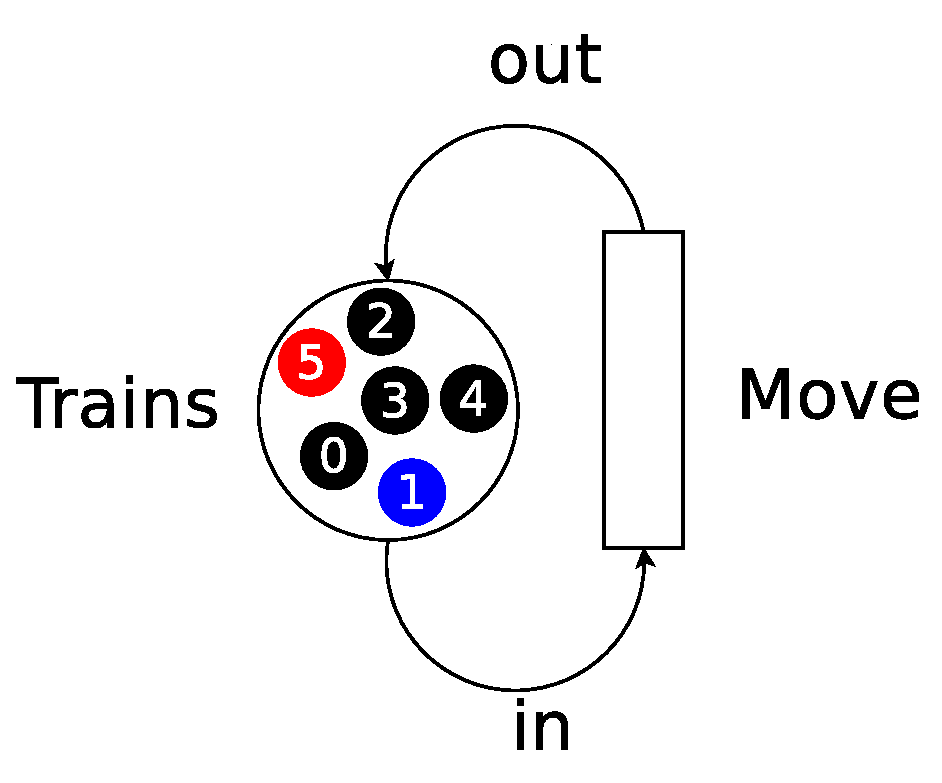
\includegraphics[height = 0.4\paperwidth]{exo8_coloured_3.eps}
\end{center}

Ici chaque couleur est une paire $c \in Trains \cup NULL \times Sectors$. 
Pour l'exemple~:

$Trains = \{ A, B\}$

$Sectors = \{0, \ldots{}, 5\}$

Les secteurs sont notés à partir de 0 et non 1 pour permettre la plus simple 
utilisation des modulo. 
Posons d'ailleurs $n\oplus{m} = (n+m)\mod{\left|Sectors\right|}$. 
Nous avons $5\oplus{1} = 0$ pour l'exemple.

$c = (T, i)$ sera noté $T_i$ par la suite. Il nous suffit de définir maintenant 
$in$ et $out$ de manière à ce que le réseau ait tous les propriétés souhaités.

Soit~:

$in(T_i) = T_{i} + NULL_{i\oplus{1}} + NULL_{i\oplus{2}}$

Et~:

$out(T_i) = NULL_{i} + T_{i\oplus{1}} + NULL_{i\oplus{2}}$

Avec bien sur $dom(in) = dom(out) = Trains \times Sectors$. Autrement dit 
$\forall i$, $in(NULL_i)$ et $out(NULL_i)$ non-définis.
